\section{CADO: Computer Aided Design Optimization Tool}
CADO is the tool of choice for engineers, designer and whoever likes to apply topology optimization on a CAD model and get a result again in CAD format. It is based on the previously described methodologies. Written in C++ and Python, this open source software is highly performant and easily expendable. CADO is straightforward to use and gives the user a one-click tool for his design optimization. In more detail, with CADO, the user only has to select a CAD input file and set the parameters. By issuing the \texttt{Run} command the tool starts the pipeline illustrated in \autoref{fig:pipeline}: 

From the given geometry (a) we start off by voxelizing (b). Next, topology optimization is applied (c) and the surface points are computed (d). After extracting the NURBS surface (e) the boolean operation is executed which results in the final geometry (f). All of this is achieved without further user interaction.
\begin{figure}[ht]
\begin{center}
		\begin{tikzpicture}[remember picture, auto,
    block/.style={
      rectangle,
      draw=blue,
      thick,
      fill=blue!20,
      text width=5em,
      align=center,
      rounded corners,
      minimum height=2em
    },
    block1/.style={
      rectangle,
      draw=blue,
      thick,
      fill=blue!20,
      text width=5em,
      align=center,
      rounded corners,
      minimum height=2em
    },
    line/.style={
      draw,thick,
      -latex',
      shorten >=2pt
    },
    cloud/.style={
      draw=red,
      thick,
      ellipse,
      fill=red!20,
      minimum height=1em
    }]
        \node [anchor=north,inner sep=0pt] [xshift=-4cm,yshift=0.7cm,inner sep=0pt](N1)
                {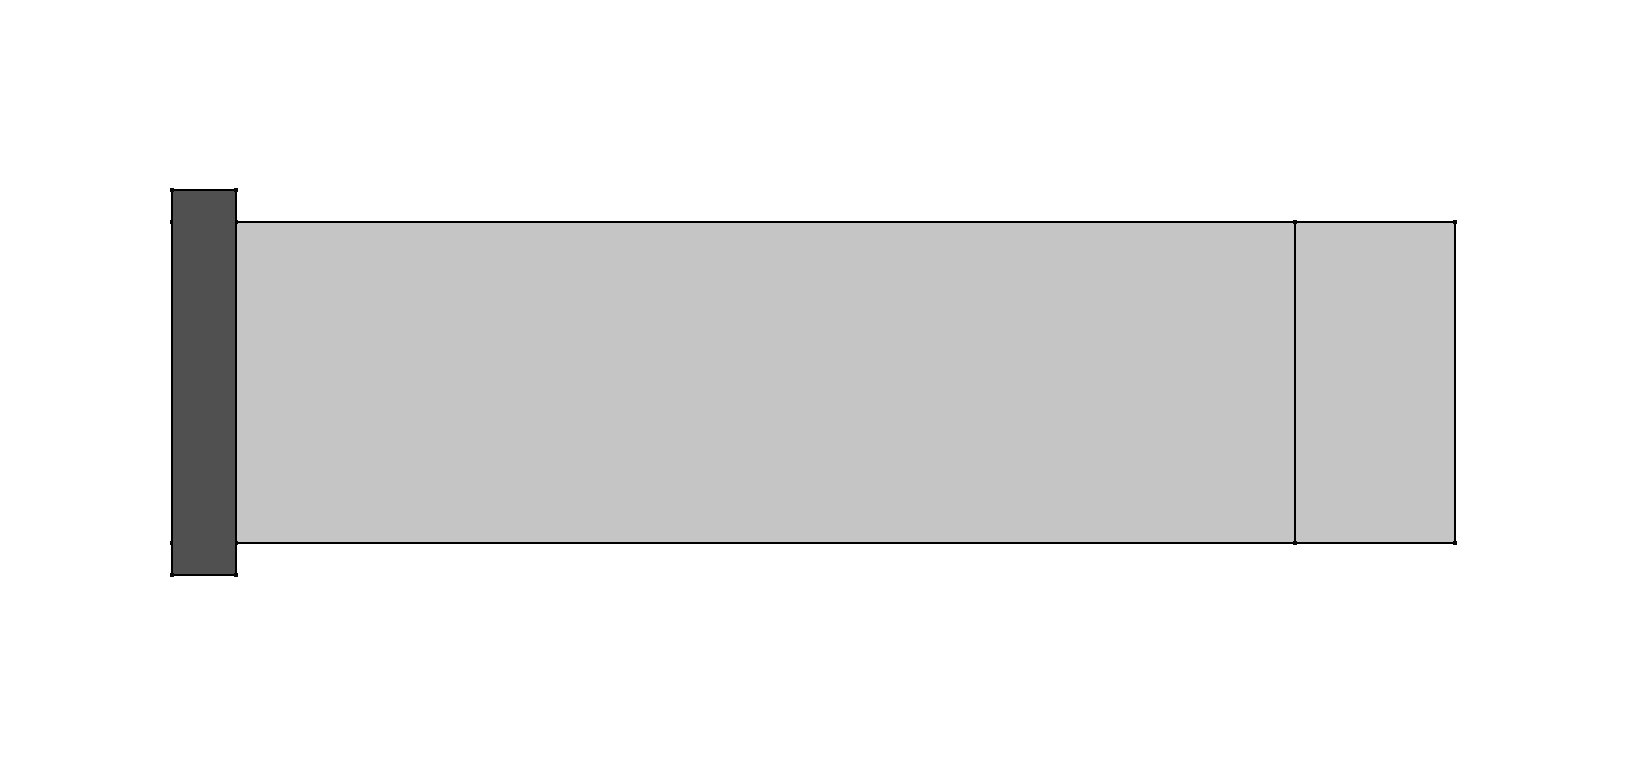
\includegraphics[scale=0.1]{Pictures/CADO_Overview/Back2CAD1.png}};
        \node [below =of N1,inner sep=0pt] [xshift=0cm,yshift=1cm,inner sep=0pt](N5)
				{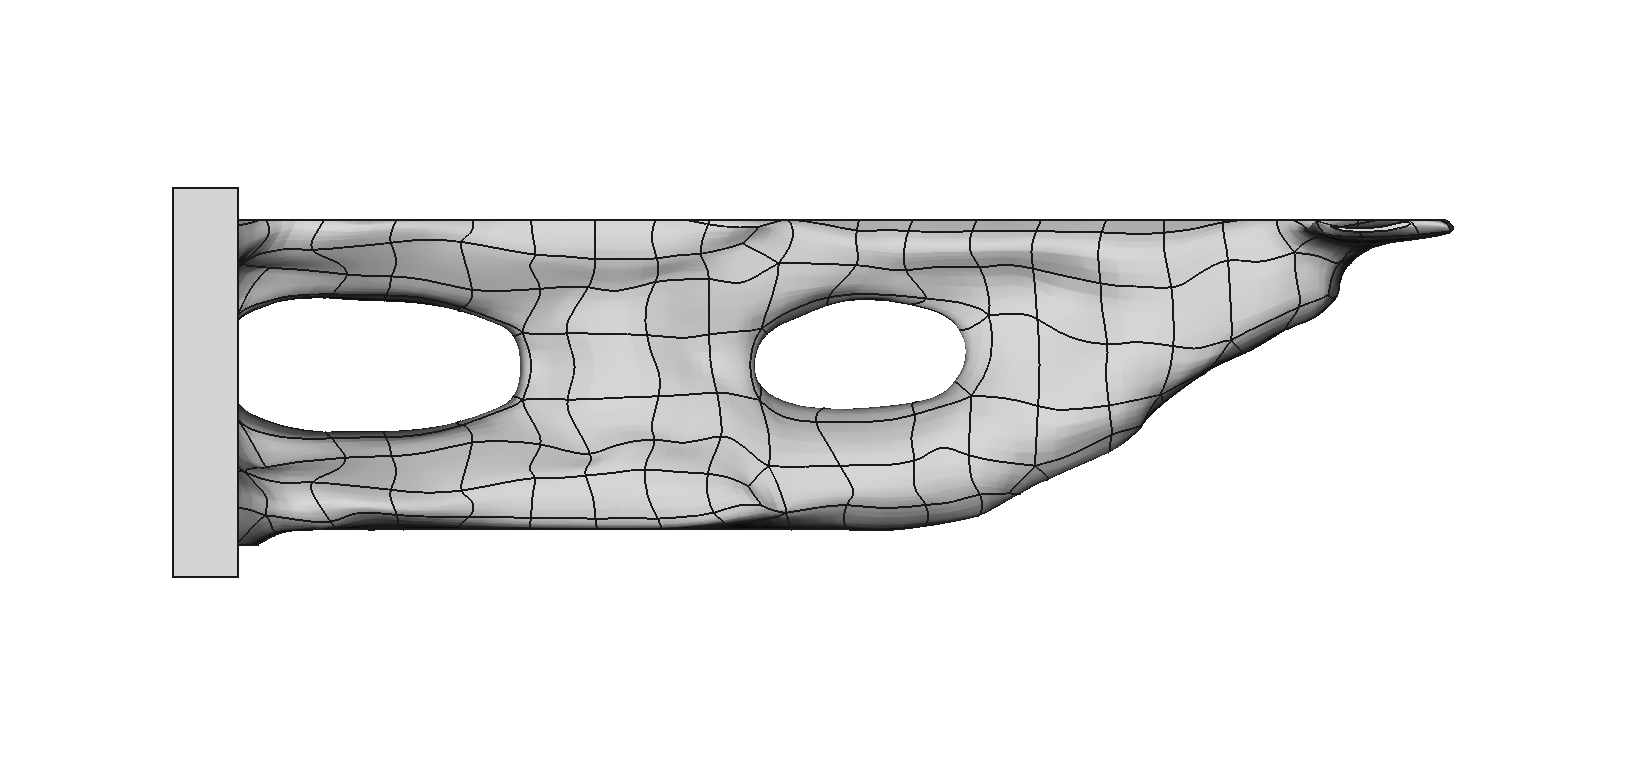
\includegraphics[scale=0.1]{Pictures/CADO_Overview/Back2CAD6.png}};
      	%\path[thick, ->,] (N5) edge [bend left] (N1); %node[yshift=-1.8cm, xshift = -0.1cm]{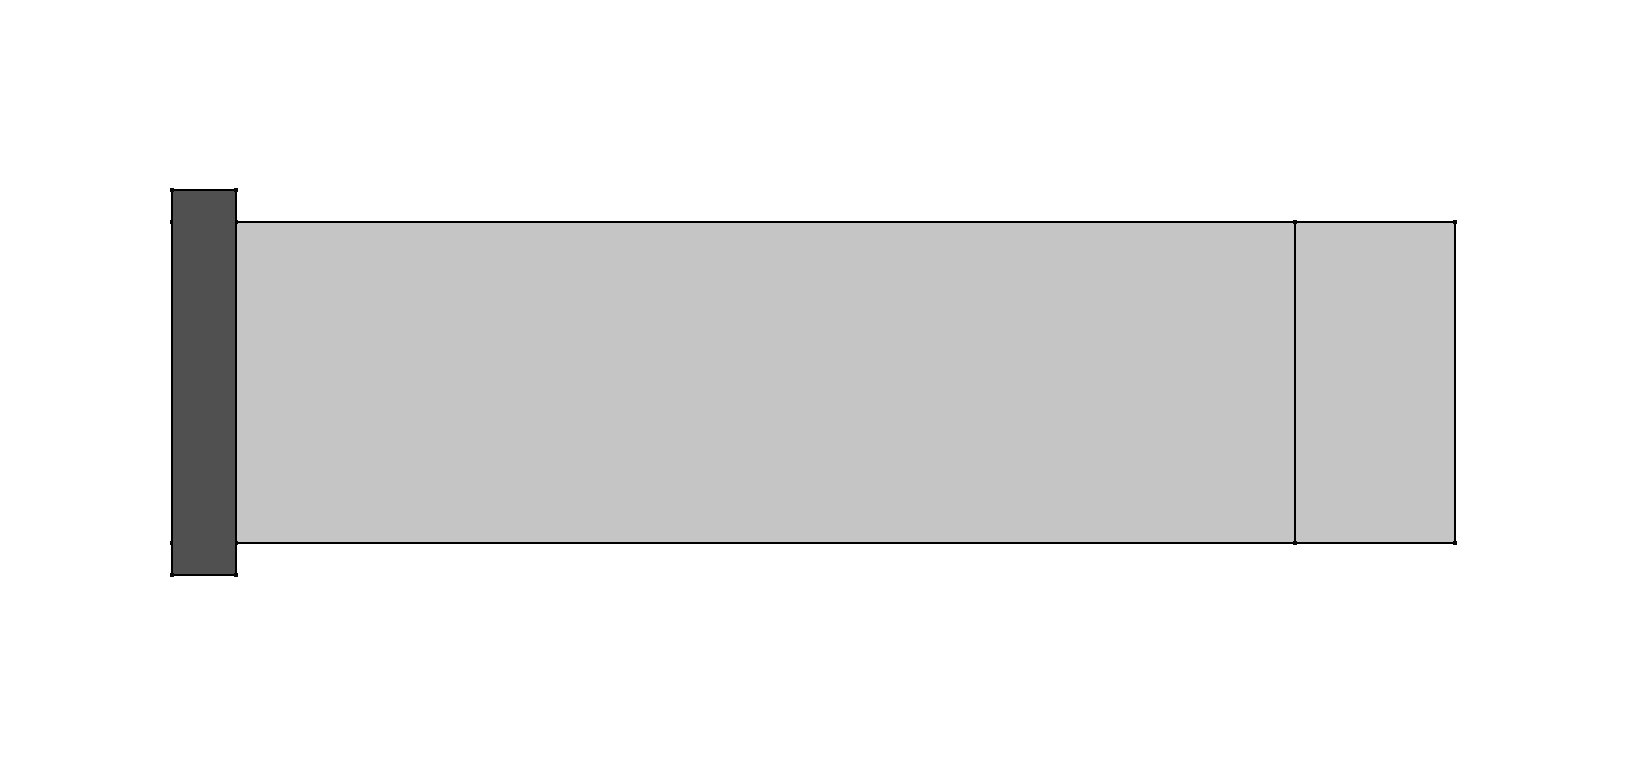
\includegraphics[scale=0.1]{Pictures/CADO_Overview/Back2CAD1.png}};
        \node [right =of N1,inner sep=0pt] [xshift=-2.5cm,yshift=2cm, inner sep=0pt](N2)             
                {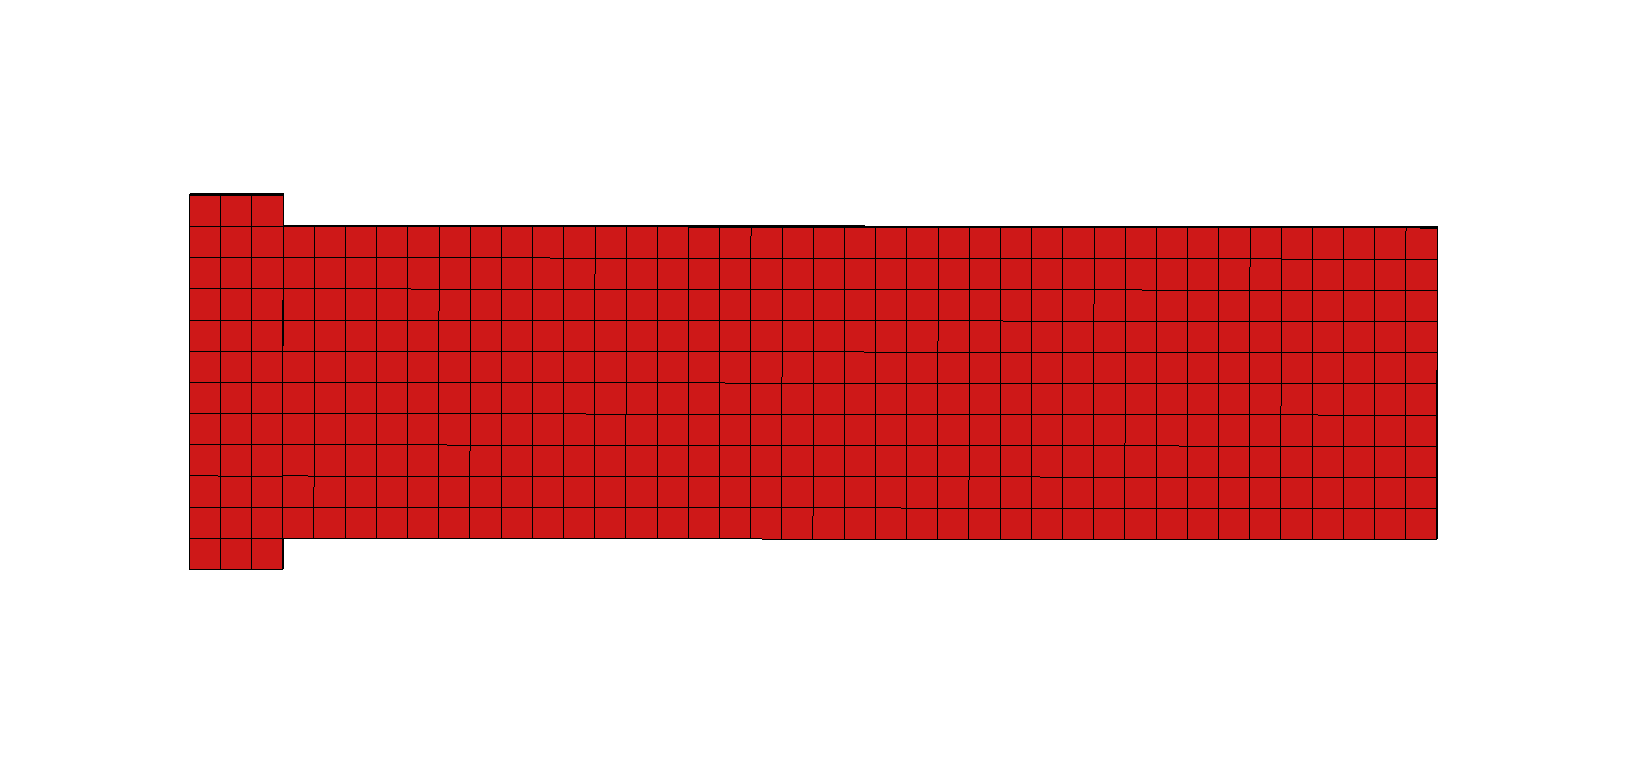
\includegraphics[scale=0.1]{Pictures/CADO_Overview/Back2CAD2.png}};
        \path[thick, ->] (N1) edge [bend left] (N2) node[yshift=0cm, xshift = -2.7cm]{(a)};
        \node [right =of N2,inner sep=0pt] [xshift=-2cm,yshift=-2cm, inner sep=0pt](N3) 
                {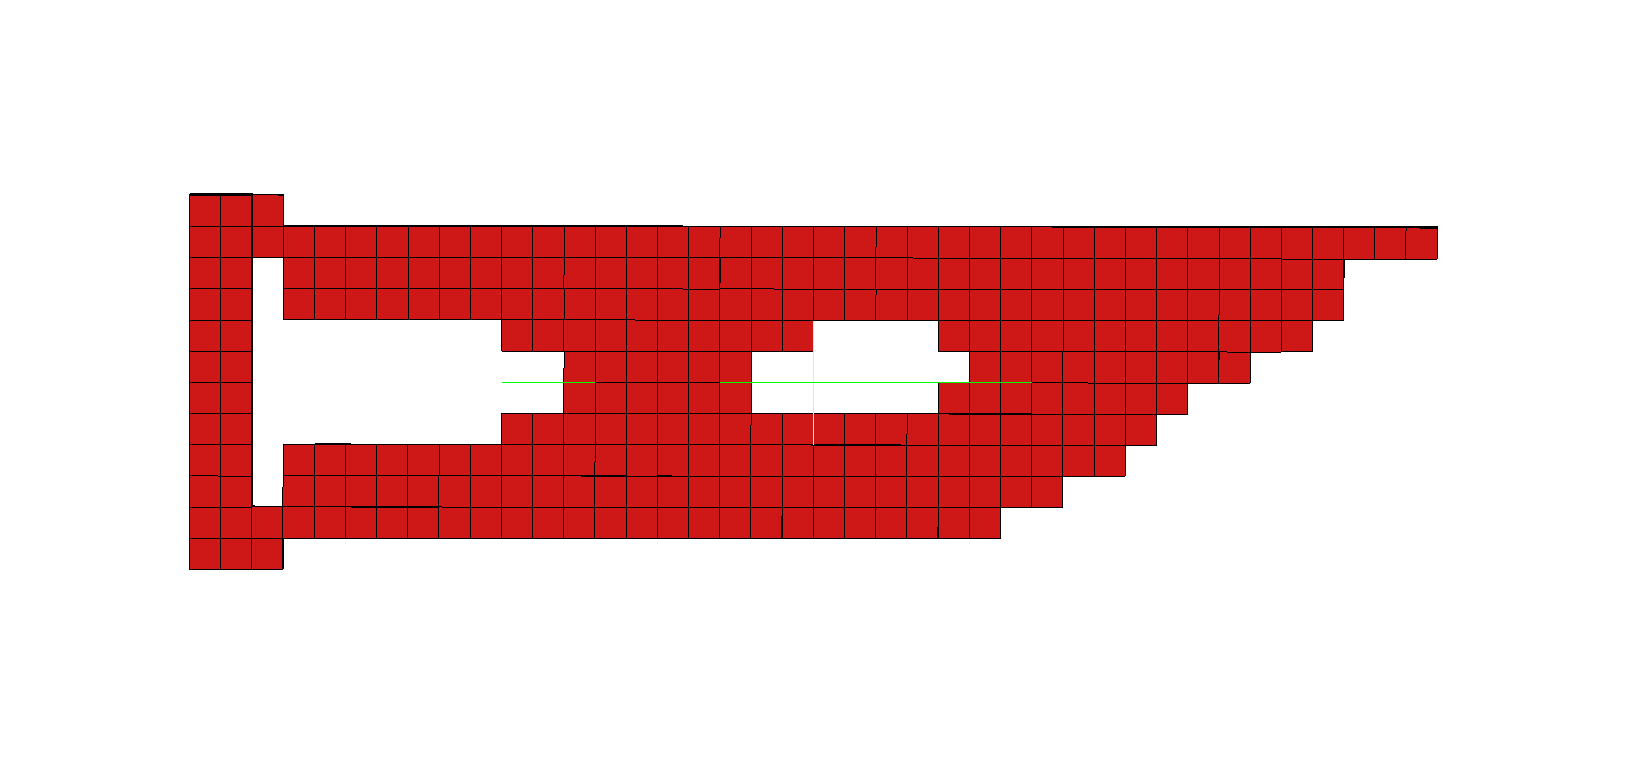
\includegraphics[scale=0.1]{Pictures/CADO_Overview/Back2CAD3.png}};
        \path[thick, ->] (N2) edge [bend left] (N3) node[yshift=1cm, xshift = 0.1cm]{(b)};
        \node [below =of N3,inner sep=0pt] [xshift=-0cm,yshift=1cm, inner sep=0pt](N4)
                {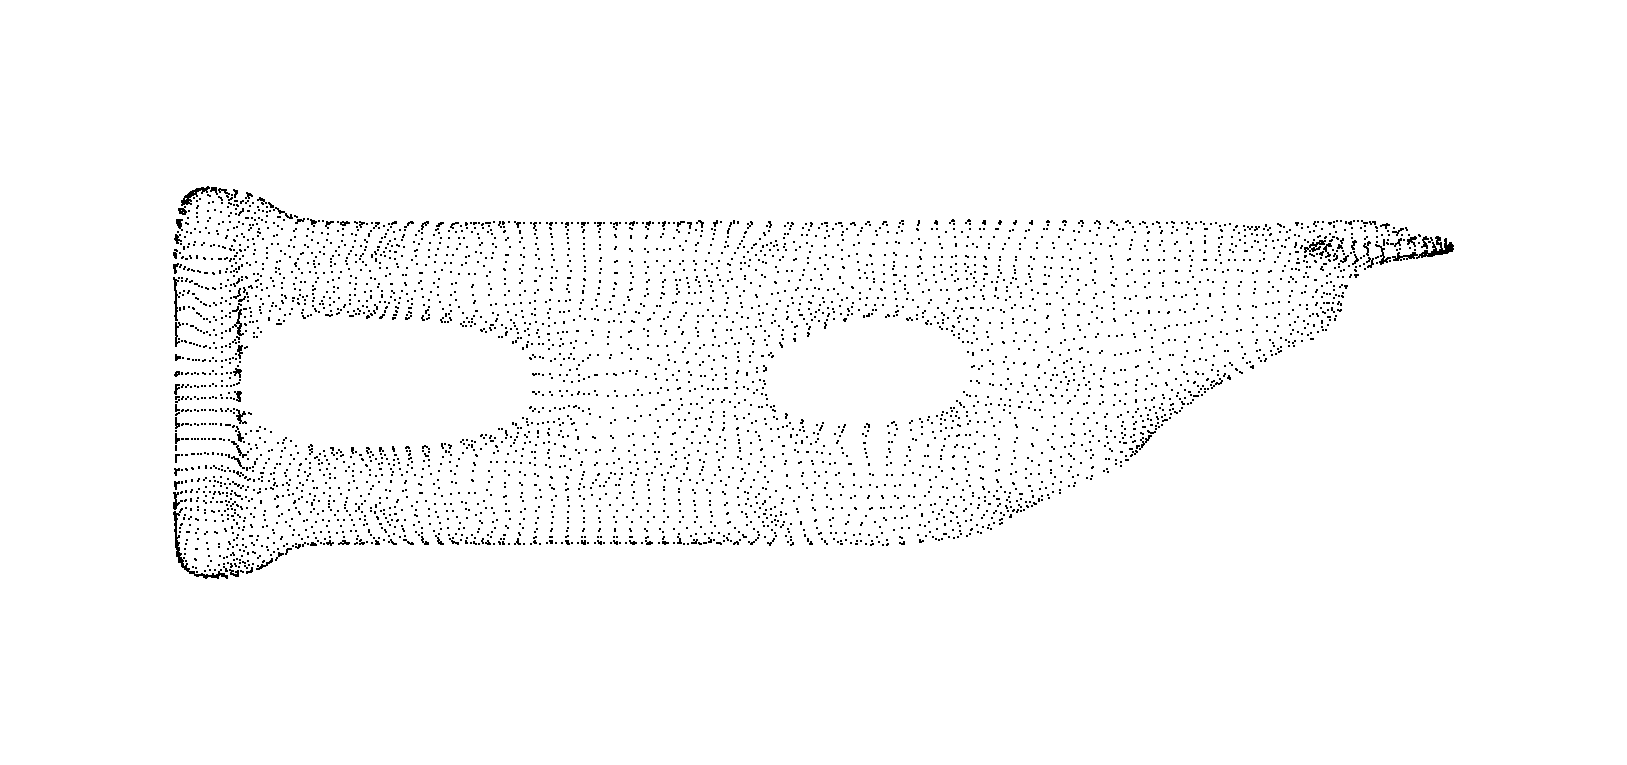
\includegraphics[scale=0.1]{Pictures/CADO_Overview/Back2CAD4.png}};
        \coordinate (N31) at (-0.9,-1);
        \coordinate (N32) at ($(N3)+(N31)$);
        \coordinate (N41) at (-0.9,1);
        \coordinate (N42) at ($(N4)+(N41)$);
        \draw[thick, ->] (N32) -- (N42) node[yshift=1.8cm, xshift = 3.5cm]{(c)};
        \node [right =of N5,inner sep=0pt] [xshift=-2.2cm,yshift=-2cm, inner sep=0pt](N6)
                {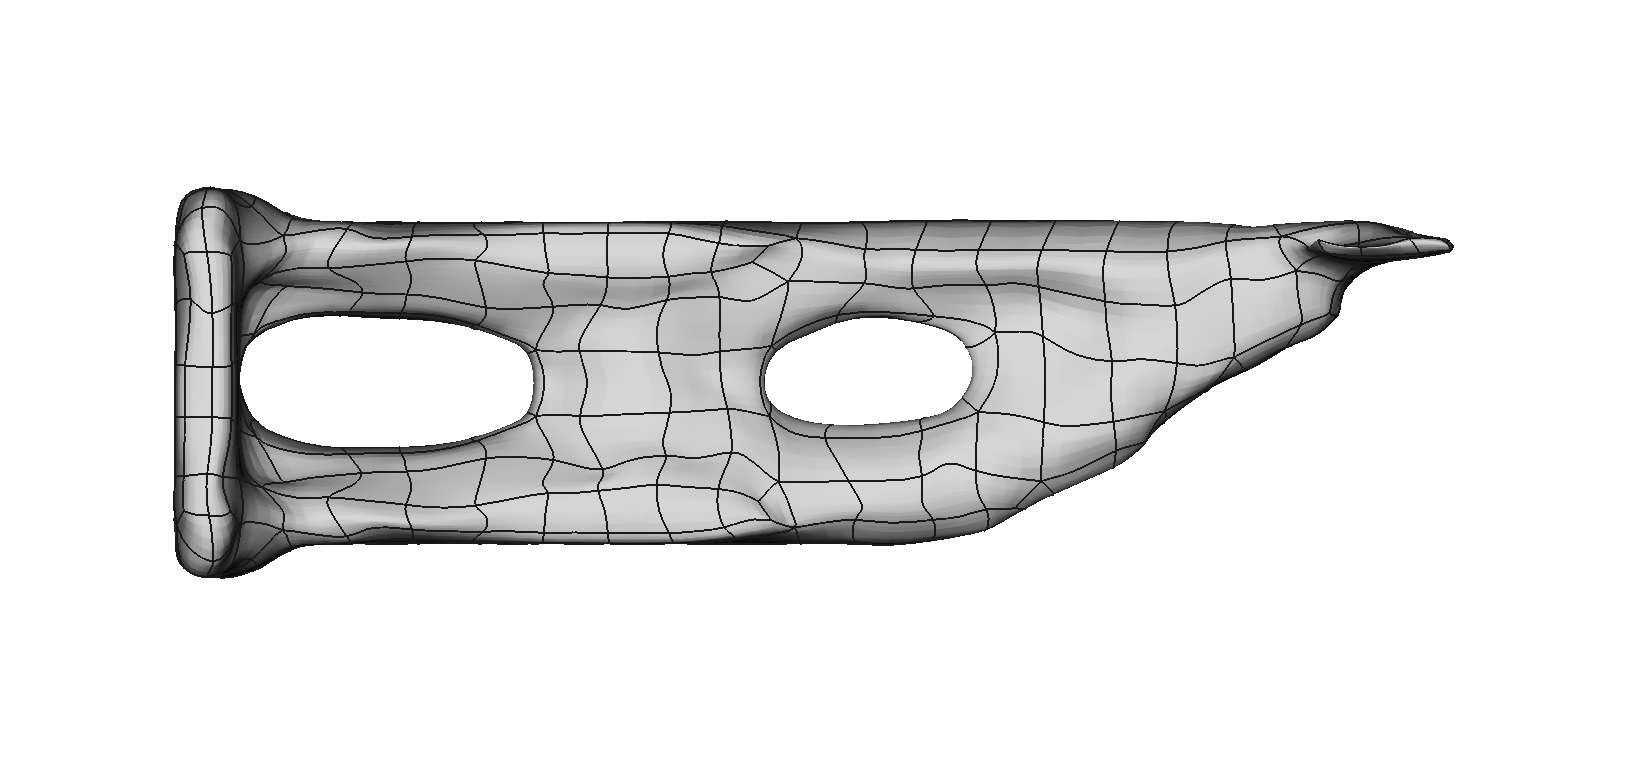
\includegraphics[scale=0.1]{Pictures/CADO_Overview/Back2CAD5.png}};
        \path[thick, ->] (N4) edge [bend left] (N6) node[yshift=0.1cm, xshift = 2.6cm]{(d)};
        \path[thick, ->] (N6) edge [bend left] (N5) node[yshift=-1cm, xshift = -0.1cm]{(e)} node[yshift=2cm, xshift = -7.22cm]{(f)};
        \end{tikzpicture}
        \caption{The workflow of CADO}
        \label{fig:pipeline}
	\end{center}
\end{figure}

The single steps of the program are completely independent and exchangeable. How they are implemented and how they collaborate is explained in the upcoming sections. CADO itself is licensed under the open source BSD license and can be found on Github \cite{CADOGit}.